\usetikzlibrary{calc}
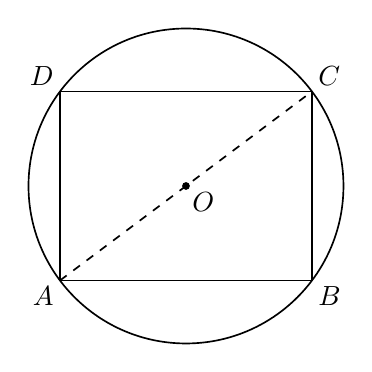
\begin{tikzpicture}[x=1cm,y=1cm,line width=.6pt,font=\normalsize]
\coordinate (O) at (0,0);
\coordinate (A) at (-1.6,-1.2);
\coordinate (B) at (1.6,-1.2);
\coordinate (C) at (1.6,1.2);
\coordinate (D) at (-1.6,1.2);
\draw (O) circle[radius=2cm];
\draw (A)--(B)--(C)--(D)--cycle;
\draw[dashed] (A)--(C);
\node[below left=2pt,inner sep=0pt] at (A) {$A$};
\node[below right=2pt,inner sep=0pt] at (B) {$B$};
\node[above right=2pt,inner sep=0pt] at (C) {$C$};
\node[above left=2pt,inner sep=0pt] at (D) {$D$};
\node[below right=2pt,inner sep=0pt] at (O) {$O$};

% Explicit named circle-center points, painted after all region fills.
\fill (O) circle[radius=1.4pt];
\end{tikzpicture}
